\documentclass[tikz,border=7pt]{standalone}
\usepackage[T1]{fontenc}
\usepackage{helvet}
\usepackage{amsmath,amssymb}
\renewcommand{\familydefault}{\sfdefault}
\usetikzlibrary{arrows.meta,positioning,fit,calc,backgrounds}

\definecolor{navy}{HTML}{17324D}
\definecolor{blue}{HTML}{2F6B9A}
\definecolor{cyan}{HTML}{DCEFF5}
\definecolor{teal}{HTML}{278C82}
\definecolor{green}{HTML}{DFF2E7}
\definecolor{orange}{HTML}{E58B3A}
\definecolor{gold}{HTML}{F8E6B6}
\definecolor{purple}{HTML}{7457A6}
\definecolor{lavender}{HTML}{E9E2F5}
\definecolor{red}{HTML}{C95555}
\definecolor{rose}{HTML}{F8E1E1}
\definecolor{ink}{HTML}{263442}
\definecolor{muted}{HTML}{607385}
\definecolor{panel}{HTML}{F6F8FA}

\begin{document}
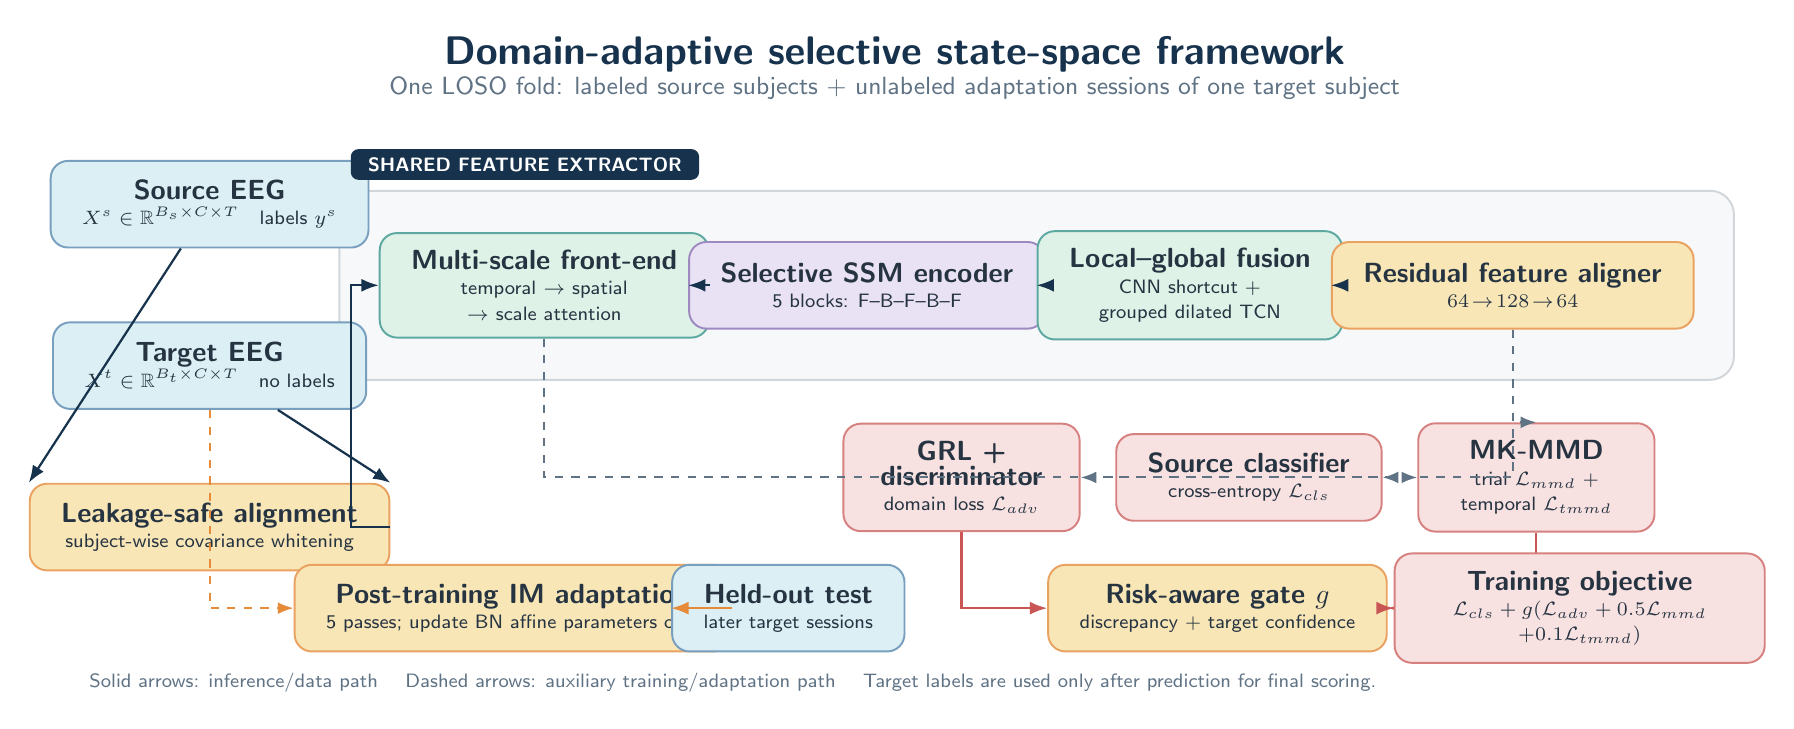
\begin{tikzpicture}[
  font=\sffamily,
  >=Latex,
  flow/.style={-{Latex[length=2.2mm]}, line width=0.8pt, draw=navy},
  aux/.style={-{Latex[length=2mm]}, line width=0.75pt, draw=muted, dashed},
  card/.style={rounded corners=2.2mm, minimum height=11mm, align=center,
               draw=navy!35, line width=0.7pt, fill=white, text=ink,
               inner xsep=4mm, inner ysep=2.2mm},
  data/.style={card, fill=cyan, draw=blue!65},
  encoder/.style={card, fill=green, draw=teal!75},
  sequence/.style={card, fill=lavender, draw=purple!70},
  adapt/.style={card, fill=gold, draw=orange!80},
  loss/.style={card, fill=rose, draw=red!75},
  tag/.style={font=\bfseries\scriptsize, text=white, rounded corners=1mm,
              inner xsep=2.2mm, inner ysep=1.1mm},
  note/.style={font=\scriptsize, text=muted, align=center}
]

% title
\node[font=\bfseries\Large, text=navy] at (10.5,7.65)
  {Domain-adaptive selective state-space framework};
\node[font=\small, text=muted] at (10.5,7.22)
  {One LOSO fold: labeled source subjects + unlabeled adaptation sessions of one target subject};

% data streams
\node[data, minimum width=3.2cm] (source) at (1.8,5.75)
  {\textbf{Source EEG}\\[-1mm]\scriptsize $X^s\in\mathbb{R}^{B_s\times C\times T}$\quad labels $y^s$};
\node[data, minimum width=3.2cm] (target) at (1.8,3.70)
  {\textbf{Target EEG}\\[-1mm]\scriptsize $X^t\in\mathbb{R}^{B_t\times C\times T}$\quad no labels};
\node[adapt, minimum width=3.2cm] (ra) at (1.8,1.65)
  {\textbf{Leakage-safe alignment}\\[-1mm]\scriptsize subject-wise covariance whitening};
\draw[flow] (source) -- (ra.north west);
\draw[flow] (target) -- (ra.north east);

% shared backbone
\node[encoder, minimum width=3.5cm] (cnn) at (6.05,4.72)
  {\textbf{Multi-scale front-end}\\[-1mm]\scriptsize temporal $\rightarrow$ spatial\\[-1mm]\scriptsize $\rightarrow$ scale attention};
\node[sequence, minimum width=3.5cm] (ssm) at (10.15,4.72)
  {\textbf{Selective SSM encoder}\\[-1mm]\scriptsize 5 blocks: F--B--F--B--F};
\node[encoder, minimum width=3.5cm] (fusion) at (14.25,4.72)
  {\textbf{Local--global fusion}\\[-1mm]\scriptsize CNN shortcut +\\[-1mm]\scriptsize grouped dilated TCN};
\node[adapt, minimum width=3.5cm] (aligner) at (18.35,4.72)
  {\textbf{Residual feature aligner}\\[-1mm]\scriptsize $64\!\rightarrow\!128\!\rightarrow\!64$};

\draw[flow] (ra.east) -| ($(cnn.west)+(-0.35,0)$) -- (cnn.west);
\draw[flow] (cnn) -- (ssm);
\draw[flow] (ssm) -- (fusion);
\draw[flow] (fusion) -- (aligner);

\begin{scope}[on background layer]
  \node[rounded corners=3mm, fill=panel, draw=navy!20, line width=0.7pt,
        fit=(cnn)(ssm)(fusion)(aligner), inner sep=5mm] (backbone) {};
\end{scope}
\node[tag, fill=navy, anchor=south west] at ($(backbone.north west)+(0.15,0.12)$)
  {SHARED FEATURE EXTRACTOR};

% heads and losses
\node[loss, minimum width=3.0cm] (cls) at (15.00,2.28)
  {\textbf{Source classifier}\\[-1mm]\scriptsize cross-entropy $\mathcal{L}_{cls}$};
\node[loss, minimum width=3.0cm] (mmd) at (18.65,2.28)
  {\textbf{MK-MMD}\\[-1mm]\scriptsize trial $\mathcal{L}_{mmd}$ +\\[-1mm]\scriptsize temporal $\mathcal{L}_{tmmd}$};
\node[loss, minimum width=3.0cm] (dann) at (11.35,2.28)
  {\textbf{GRL +}\\[-1mm]\textbf{discriminator}\\[-1mm]\scriptsize domain loss $\mathcal{L}_{adv}$};
\node[adapt, minimum width=3.4cm] (gate) at (14.60,0.62)
  {\textbf{Risk-aware gate $g$}\\[-1mm]\scriptsize discrepancy + target confidence};

\draw[aux] (aligner.south) |- (cls.east);
\draw[aux] (aligner.south) |- (mmd.north);
\draw[aux] (aligner.south) |- (dann.east);
\draw[aux] (cnn.south) |- (mmd.west);
\draw[flow, draw=red] (dann.south) |- (gate.west);
\draw[flow, draw=red] (mmd.south) |- (gate.east);

\node[loss, minimum width=4.7cm] (objective) at (19.20,0.62)
  {\textbf{Training objective}\\[-1mm]\scriptsize $\mathcal{L}_{cls}+g(\mathcal{L}_{adv}+0.5\mathcal{L}_{mmd}$\\[-1mm]\scriptsize $+0.1\mathcal{L}_{tmmd})$};
\draw[flow, draw=red] (gate) -- (objective);

% post-training path
\node[adapt, minimum width=3.65cm] (imtta) at (5.65,0.62)
  {\textbf{Post-training IM adaptation}\\[-1mm]\scriptsize 5 passes; update BN affine parameters only};
\node[data, minimum width=2.75cm] (test) at (9.15,0.62)
  {\textbf{Held-out test}\\[-1mm]\scriptsize later target sessions};
\draw[aux, draw=orange] (target.south) |- (imtta.west);
\draw[flow, draw=orange] (imtta) -- (test);

% annotations
\node[note, anchor=west] at (0.15,-0.32)
  {Solid arrows: inference/data path \quad Dashed arrows: auxiliary training/adaptation path \quad Target labels are used only after prediction for final scoring.};

\end{tikzpicture}
\end{document}
